\documentclass{article}

\usepackage{ctex}% 导入中文宏包
\usepackage{array}
\usepackage{caption}
\usepackage{float}
\usepackage{hyperref}
% 设置页面边距
\usepackage{geometry}
\usepackage{graphicx}
\geometry{a4paper, left=2.5cm, right=2.5cm, top=3cm, bottom=3cm}

% 设置标题、作者和日期
\title{Latex与Git}
\author{23020007030  关嘉琪}

\begin{document}
	
	% 生成标题、作者和日期
	\maketitle
	
	% 报告正文
	\section{实验目的}
	本次课程主要讲授了版本控制(Git)以及Latex文档编辑,通过对两者的学习来加强对两大便捷工具的使用
	
	\section{介绍}
	\subsection{两大工具的优点}
	Git是一个开源的分布式版本控制系统,可以有效、高速地处理从很小到非常大的项目版本管理。也是Linus Torvalds为了帮助管理Linux内核开发而开发的一个开放源码的版本控制软件。
	
	LaTeX原名TeX,是一种基于TeX的排版系统,用于生成专业排版的高质量文档。它提供了对复杂的数学公式、 ID标签和脚注等的强大支持,被广泛应用于学术界、出版业和其他需要精确排版的领域。
	
	通过 Git 和 LaTeX,可以自动化文档的构建和部署过程,确保文档的一致性和准确性。
	\section{实验内容}
	\subsection{Latex学习例子10个}
	
	\begin{verbatim}
		 1.\chapter{} 章节题目
		   \section{} 标题
		   \subsection{} 小部分
		   \subsubsection{}更小的部分  从上往下层级依次细化
	\end{verbatim}
	
	2. \verb|\verb命令里面||里面可以放入想表示的指令,这样它就会以文本的方式输出|
	
	3.begin[]和end[]可以构成环境,在里面可以编写内容。
	\begin{verbatim}
		begin[itemize]和end[itemize]构成无序列表,begin[enumerate]和end[enumerate]构成有序列表
		下面是例子:
	\end{verbatim}
	\begin{enumerate}
		\item 有序列表
		//有序列表,指有序号
	\end{enumerate}%有序列表,指有序号
	\begin{itemize}
		\item 无序列表
		//无序列表,指无序号
	\end{itemize}%无序列表,指无序号
	
	4.\verb|includegraphics[width=\textwidth]{}|该命令可以用来引入图片
	\begin{figure}[H]
		\centering % 使图片居中
		\includegraphics[height = 5cm, width=\textwidth]{"example1.png"}
		\caption{这是第二个例子的图片。} % 图片的标题
		\label{fig:example} % 为图片设置标签,以便引用
	\end{figure}
	
	5.\verb|\newline的功能是换行,可以使用 \newline 命令来实现换行。这个命令会将当前位置设置为新的一行|
	
	6.\verb|\usepackage{}可以用来引入宏包或者设置字体编码下面是几个例子|\begin{verbatim}
		\usepackage[utf8]{inputenc}  % 设置输入编码
		\usepackage[T1]{fontenc}     % 设置字体编码
		\usepackage{graphicx}        % 插入图片
		\usepackage{amsmath}         % 数学公式
		\usepackage{amsfonts}        % 数学字体
		\usepackage{amssymb}         % 数学符号
		\usepackage{hyperref}        % 超链接
	\end{verbatim}
	
	7.\verb|创建表格的命令\hline|
	
	\begin{tabular}{|l|c|r|}
		\hline
		Column 1 & Column 2 & Column 3 \\
		\hline
		Left & Center & Right \\
		\hline
	\end{tabular}
	\newline
	
	8.
	\verb|\footnote{}可以添加脚注|
	
	This is a text with a footnote\footnote{This is the footnote.}.
	
	9.
	\verb|\textbf{}是加粗,\textit{}是倾斜,\underline{}是加下划线|
	
	This is \textbf{textbf}, this is \textit{textit}, and this is \underline{underlined}.
	
	
	
	10.\verb|\title是加题目|\title{My Simple Document} 
	
	\verb|\author是加作者|\author{Jane Doe}
	   
	\verb|\date|是加日期|\date{\today}
	
	\subsection{Git学习例子10个}
	1.初始化新仓库:git init
	
	\noindent
	\begin{minipage}{\linewidth}
		\centering
		% 插入图片
		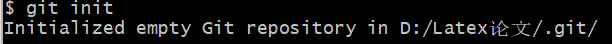
\includegraphics[width=0.5\linewidth]{example2.png}
		% 图片标题
		\captionof{figure}{初始化新仓库}
		\label{fig:example}
	\end{minipage}
	
	
	2.添加文件:git add .
	
	
	\noindent
	\begin{minipage}{\linewidth}
		\centering
		% 插入图片
		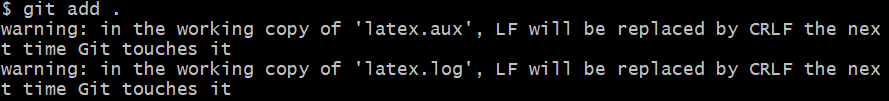
\includegraphics[width=0.5\linewidth]{example3.png}
		% 图片标题
		\captionof{figure}{添加文件}
		\label{fig:example}
	\end{minipage}
	
	3.将你的 LaTeX 源文件添加到 Git 仓库:git commit -m "Initial commit of LaTeX project"
	
	\noindent
	\begin{minipage}{\linewidth}
		\centering
		% 插入图片
		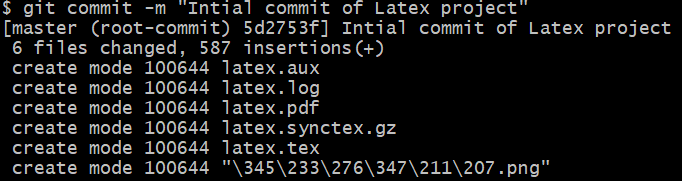
\includegraphics[width=0.5\linewidth]{example4.png}
		% 图片标题
		\captionof{figure}{将Latex源文件添加到Git仓库}
		\label{fig:example}
	\end{minipage}
	
	4.查看工作目录和暂存区的状态:git status
	
	\noindent
	\begin{minipage}{\linewidth}
	\centering
	% 插入图片
	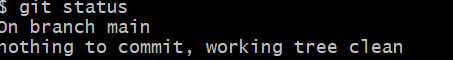
\includegraphics[width=0.5\linewidth]{example6.png}
	% 图片标题
	\captionof{figure}{查看工作目录和暂存区状态}
	\label{fig:example}
	\end{minipage}
	
	5.在处理大型文档或尝试新功能时,可以创建分支来隔离开发工作。
	git checkout -b feature-branch
	
	\noindent
	\begin{minipage}{\linewidth}
		\centering
		% 插入图片
		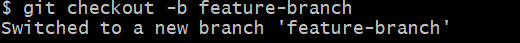
\includegraphics[width=0.5\linewidth]{example5.png}
		% 图片标题
		\captionof{figure}{创建分支}
		\label{fig:example}
	\end{minipage}
	
	6.列出所有分支:git branch
	
	\noindent
	\begin{minipage}{\linewidth}
		\centering
		% 插入图片
		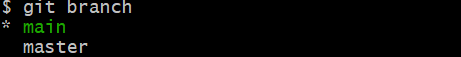
\includegraphics[width=0.5\linewidth]{example7.png}
		% 图片标题
		\captionof{figure}{初始化新仓库}
		\label{fig:example}
	\end{minipage}
	
	7.展示历来提交版本:git log
	
	\noindent
	\begin{minipage}{\linewidth}
		\centering
		% 插入图片
		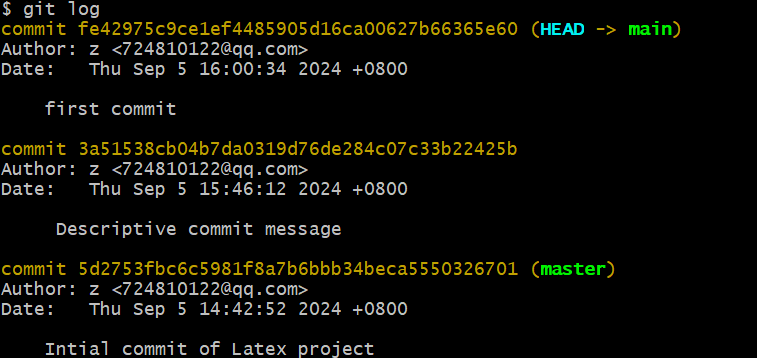
\includegraphics[width=0.5\linewidth]{example8.png}
		% 图片标题
		\captionof{figure}{展示历来提交版本}
		\label{fig:example}
	\end{minipage}
	
	8.打开任意版本:git show hash(哈希值)
	
	\noindent
	\begin{minipage}{\linewidth}
		\centering
		% 插入图片
		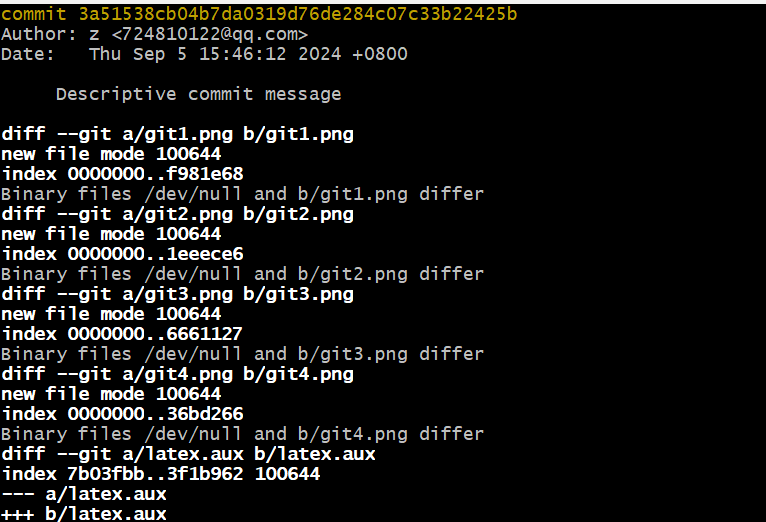
\includegraphics[width=0.5\linewidth]{example9.png}
		% 图片标题
		\captionof{figure}{打开任意版本}
		\label{fig:example}
	\end{minipage}
	
	9. 将当前分支回退到指定的提交:git reset --hard [commit hash]
	
	此处不做展示
	
	10.查看工作目录和暂存区之间的差异:git diff
	
	\noindent
	\begin{minipage}{\linewidth}
		\centering
		% 插入图片
		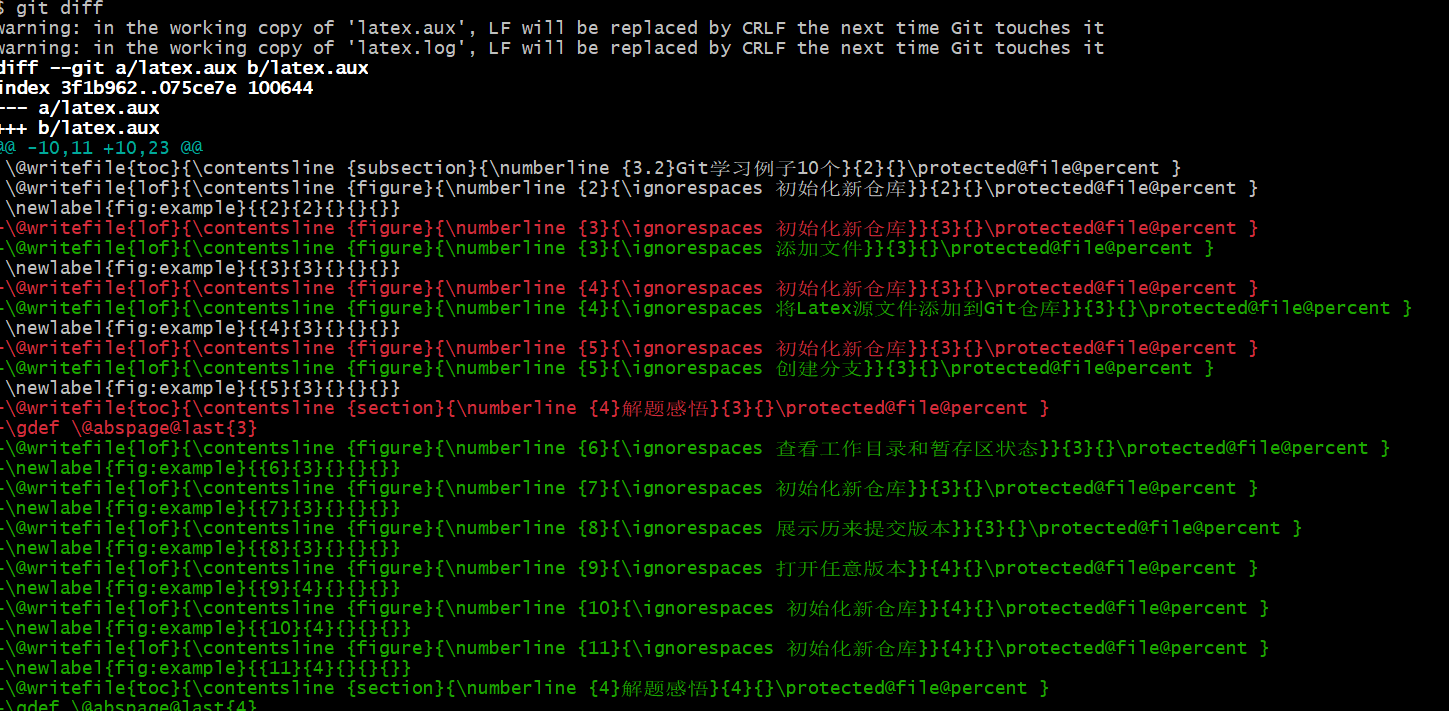
\includegraphics[width=0.5\linewidth]{example10.png}
		% 图片标题
		\captionof{figure}{查看工作目录和暂存区之间的差异}
		\label{fig:example}
	\end{minipage}
	
	
	
	
	\section{实验总结}
	通过学习LaTeX,我获得了制作格式规范且排版美观文档的能力。写实验报告时,我能够将更多精力投入到内容创作上,而不必过多关注文档的格式问题。此外,LaTeX在处理数学公式和科学符号方面的强大功能,使其成为学术写作和科学交流的理想工具。利用LaTeX,我可以通过代码轻松地进行文档的维护和修改,提升了工作效率。
	
	与此同时,Git教会了我如何有效管理代码的历史版本,这对提高工作效率至关重要。我首先学习了如何进行分支管理,以及如何进行代码的备份与恢复,这让我即使在本地文件丢失的情况下,也能从远程仓库中找回我的文件。当我遇到合并冲突或其他技术问题时,Git促使我深入分析问题并寻找解决方案,这不仅增强了我的技术能力,也提升了我的问题解决能力。
	
	github路径:
	
	\url{https://github.com/Joyceapple/repo/tree/1df1364fe4dbf130e2856605d9c21002f3045396/Latex_git}
\end{document}
